\documentclass[11pt]{article}
\usepackage[margin=1in]{geometry}
\usepackage[hidelinks]{hyperref}
\usepackage{graphicx}
\usepackage{booktabs}
\usepackage{listings}
\usepackage{xcolor}

\lstset{
  basicstyle=\ttfamily\small,
  breaklines=true,
  frame=single,
  backgroundcolor=\color{gray!8},
}

\title{\textbf{FluctlightDB: A Memory Model of Data for AI Agents}\\[0.4em]
\large A brain-native database engine for long-term agent memory}
\author{Ganesh S\\ \small Independent Researcher \quad \texttt{voxmastery@gmail.com}\\[0.2em]
\small ORCID: \href{https://orcid.org/0009-0006-7758-4114}{0009-0006-7758-4114}}
\date{June 2026}

\begin{document}
\maketitle

\begin{abstract}
For fifty years, data systems have answered two questions. The relational model
asked \emph{which records match a predicate}; the vector model asked \emph{which
vectors lie nearest a query}. Neither was built to answer the question an
autonomous agent asks every time it wakes up: \emph{what have I learned, and what
of it can I trust?} We argue that long-term agent memory is not an application
built on top of a database---it is a \textbf{third data model}, with its own write
semantics (encoding, separation, consolidation, provenance) and its own read
semantics (cue-driven activation across a linked memory graph). We present
\textbf{FluctlightDB}, an embedded, brain-native database engine that implements
this model behind two primitives, \texttt{experience()} and \texttt{activate()}.
On the official LoCoMo long-conversation benchmark (10 conversations,
1{,}982 gold evidence spans), FluctlightDB's hybrid index recalls \textbf{98.1\%}
of gold evidence---warm and cold-start identical. On LongMemEval-S (500 questions,
official \texttt{session\_recall@8}), our retrieval harness scores \textbf{98.0\%}
(490/500), competitive with published hybrid memory systems on the same benchmark.
On BEIR SciFact it matches a tuned Chroma + MiniLM baseline on nDCG@10 at equal
latency, while agent mode improves Recall@100. On an agent-specific suite (FAMB)
it scores 97--98\% macro across paraphrase recall, provenance ranking,
persistence, and write-time separation. The engine, harnesses, and frozen metrics
are released under the MIT license. We claim no new neuroscience and no new
transformer; we claim a missing layer of the data stack, and an engine that fills it.
\end{abstract}

\section{Introduction}
Every generation of software gets the database it deserves. Business records gave
us the relational model~\cite{codd1970relational} and SQL. Embeddings gave us
vector databases and approximate nearest-neighbor search. Agents---programs that
act, observe, and persist across sessions---have so far been handed \emph{neither}.
They are stateless between runs unless a developer hand-assembles a session store,
a vector index, a deduplicator, a trust policy, and glue code to keep them
consistent. The result is that ``memory'' for agents lives in application code,
re-implemented badly in every project, with no shared abstraction and no
benchmark to hold it accountable.

This paper makes a deliberately large claim and then defends it with measurements:
\textbf{agent memory deserves its own database engine, not a wrapper around someone
else's.} A relational engine is the wrong abstraction because memory is not a set
of typed rows joined by keys. A vector engine is the wrong abstraction because
recall is not cosine similarity alone---a human, and an agent, retrieve a fact
because it was \emph{learned}, \emph{linked} to a context, and \emph{trusted},
not merely because its embedding is close. What is missing is a model whose unit
is the \emph{episode}---an experience with content, context, salience, and
provenance---and whose query is a \emph{cue} that spreads through associations.

\textbf{Contributions.}
\begin{itemize}
  \item \textbf{A data model.} We define agent memory as a first-class model of
  data with explicit write semantics (separation, encoding, consolidation,
  provenance) and read semantics (cue activation over a memory graph), distinct
  from the relational and vector models.
  \item \textbf{An engine.} FluctlightDB, an embedded Rust engine exposing
  \texttt{experience()} / \texttt{activate()} / \texttt{checkpoint()}---one
  durable store per agent, with no external services.
  \item \textbf{Evidence.} \textbf{98.1\%} evidence recall on full LoCoMo,
  \textbf{98.0\%} session recall@8 on LongMemEval-S (composite full run + v4
  preference slice), parity with a tuned
  vector baseline on BEIR SciFact, and 97--98\% macro on an agent-specific
  benchmark.
  \item \textbf{Reproducibility.} Open harnesses and frozen result JSON so every
  number here can be re-run with one command.
\end{itemize}

\section{The Third Data Model}
\subsection{Why rows are not memory}
The relational model stores facts whose schema is known in advance and whose
truth is uniform. Agent memory is the opposite: heterogeneous, arriving out of
order, often contradictory (a chat claim vs.\ a ledger entry), and valuable
precisely \emph{because} of where it came from. SQL has no native notion of
provenance-weighted recall or of an experience that should be down-weighted
because a more trusted source disagrees.

\subsection{Why nearest-neighbor is not recall}
Vector search answers ``what is similar.'' Memory answers ``what is relevant given
who I am and what I was doing.'' Two memories with distant embeddings can be the
right answer because they were co-activated during the same episode; a near
embedding can be the wrong answer because it is an unverified rumor. Pure ANN has
no place to encode association strength, salience decay, or trust.

\subsection{The model}
We define a memory store as a set of \emph{engrams}. Each engram carries content,
an encoding context, a salience weight, optional provenance, and edges to
co-activated engrams. The write operation \texttt{experience} performs pattern
\emph{separation} (near-duplicates are gated, not blindly appended), encodes the
engram, registers its semantic vector, and wires graph edges. The read operation
\texttt{activate} takes a cue, seeds both lexical and semantic indexes, spreads
activation through the graph, fuses the scores, and applies provenance boosts so
verified sources outrank chat. Consolidation replays and compacts the store
offline, the way sleep consolidates biological memory. This is the entire
contract; the neuroscience vocabulary is explanatory, not required to use it.

\begin{table}[h]
\centering
\caption{Brain-native primitives vs.\ relational and vector abstractions.}
\begin{tabular}{p{2.2cm}p{4.2cm}p{4.8cm}}
\toprule
\textbf{Primitive} & \textbf{Role in FluctlightDB} & \textbf{Relational / vector analogue} \\
\midrule
Engram & Unit of memory: content, context, salience, provenance, edges & Row; or embedded chunk \\
\texttt{experience()} & Write: separation, encode, index, wire co-activation & \texttt{INSERT} / upsert \\
\texttt{activate(cue)} & Read: lexical + semantic seed, graph spread, fusion, trust boost & \texttt{SELECT} / ANN top-$k$ \\
Consolidation & Offline replay and compaction (\texttt{checkpoint()}) & Vacuum / reindex only \\
Provenance & Verified sources outrank unverified chat at recall & No native type \\
\bottomrule
\end{tabular}
\end{table}

\section{System Design}
\subsection{Embedded, one store per agent}
Like SQLite, FluctlightDB is a library, not a server: each agent owns a directory
on disk and \texttt{checkpoint()} commits state. There is nothing to provision and
nothing to keep in sync. A thin HTTP server is provided for multi-agent
deployments but is not required.

\subsection{Write path}
Incoming \texttt{experience} episodes pass through optional separation gating,
dentate-style encoding into engrams, semantic vector registration, and graph
wiring. A fast-ingest mode skips heavy graph work for bulk indexing.

\subsection{Read path}
\texttt{activate(cue)} seeds lexical (BM25) and semantic (vector) indexes, spreads
activation through the memory graph, fuses scores, and applies provenance boosts.
For conversational RAG we merge vector top-$k$ with lexical seeds---\emph{hybrid
retrieval}---before ranking. A vector-fast mode provides Chroma-class cosine
top-$k$ for IR comparisons.

\subsection{Two explicit modes}
\texttt{connect()} is the full episodic engine (separation, graph, provenance) for
live agents. \texttt{connect\_index()} is the bulk semantic path for RAG backfills
and IR benchmarks. The modes share one engine and one file format.

Figure~\ref{fig:architecture} summarizes how an agent brain is laid out on disk,
what each engram stores, and how write and read paths connect the episodic store
to the hybrid recall sidecar.

\begin{figure*}[t]
\centering
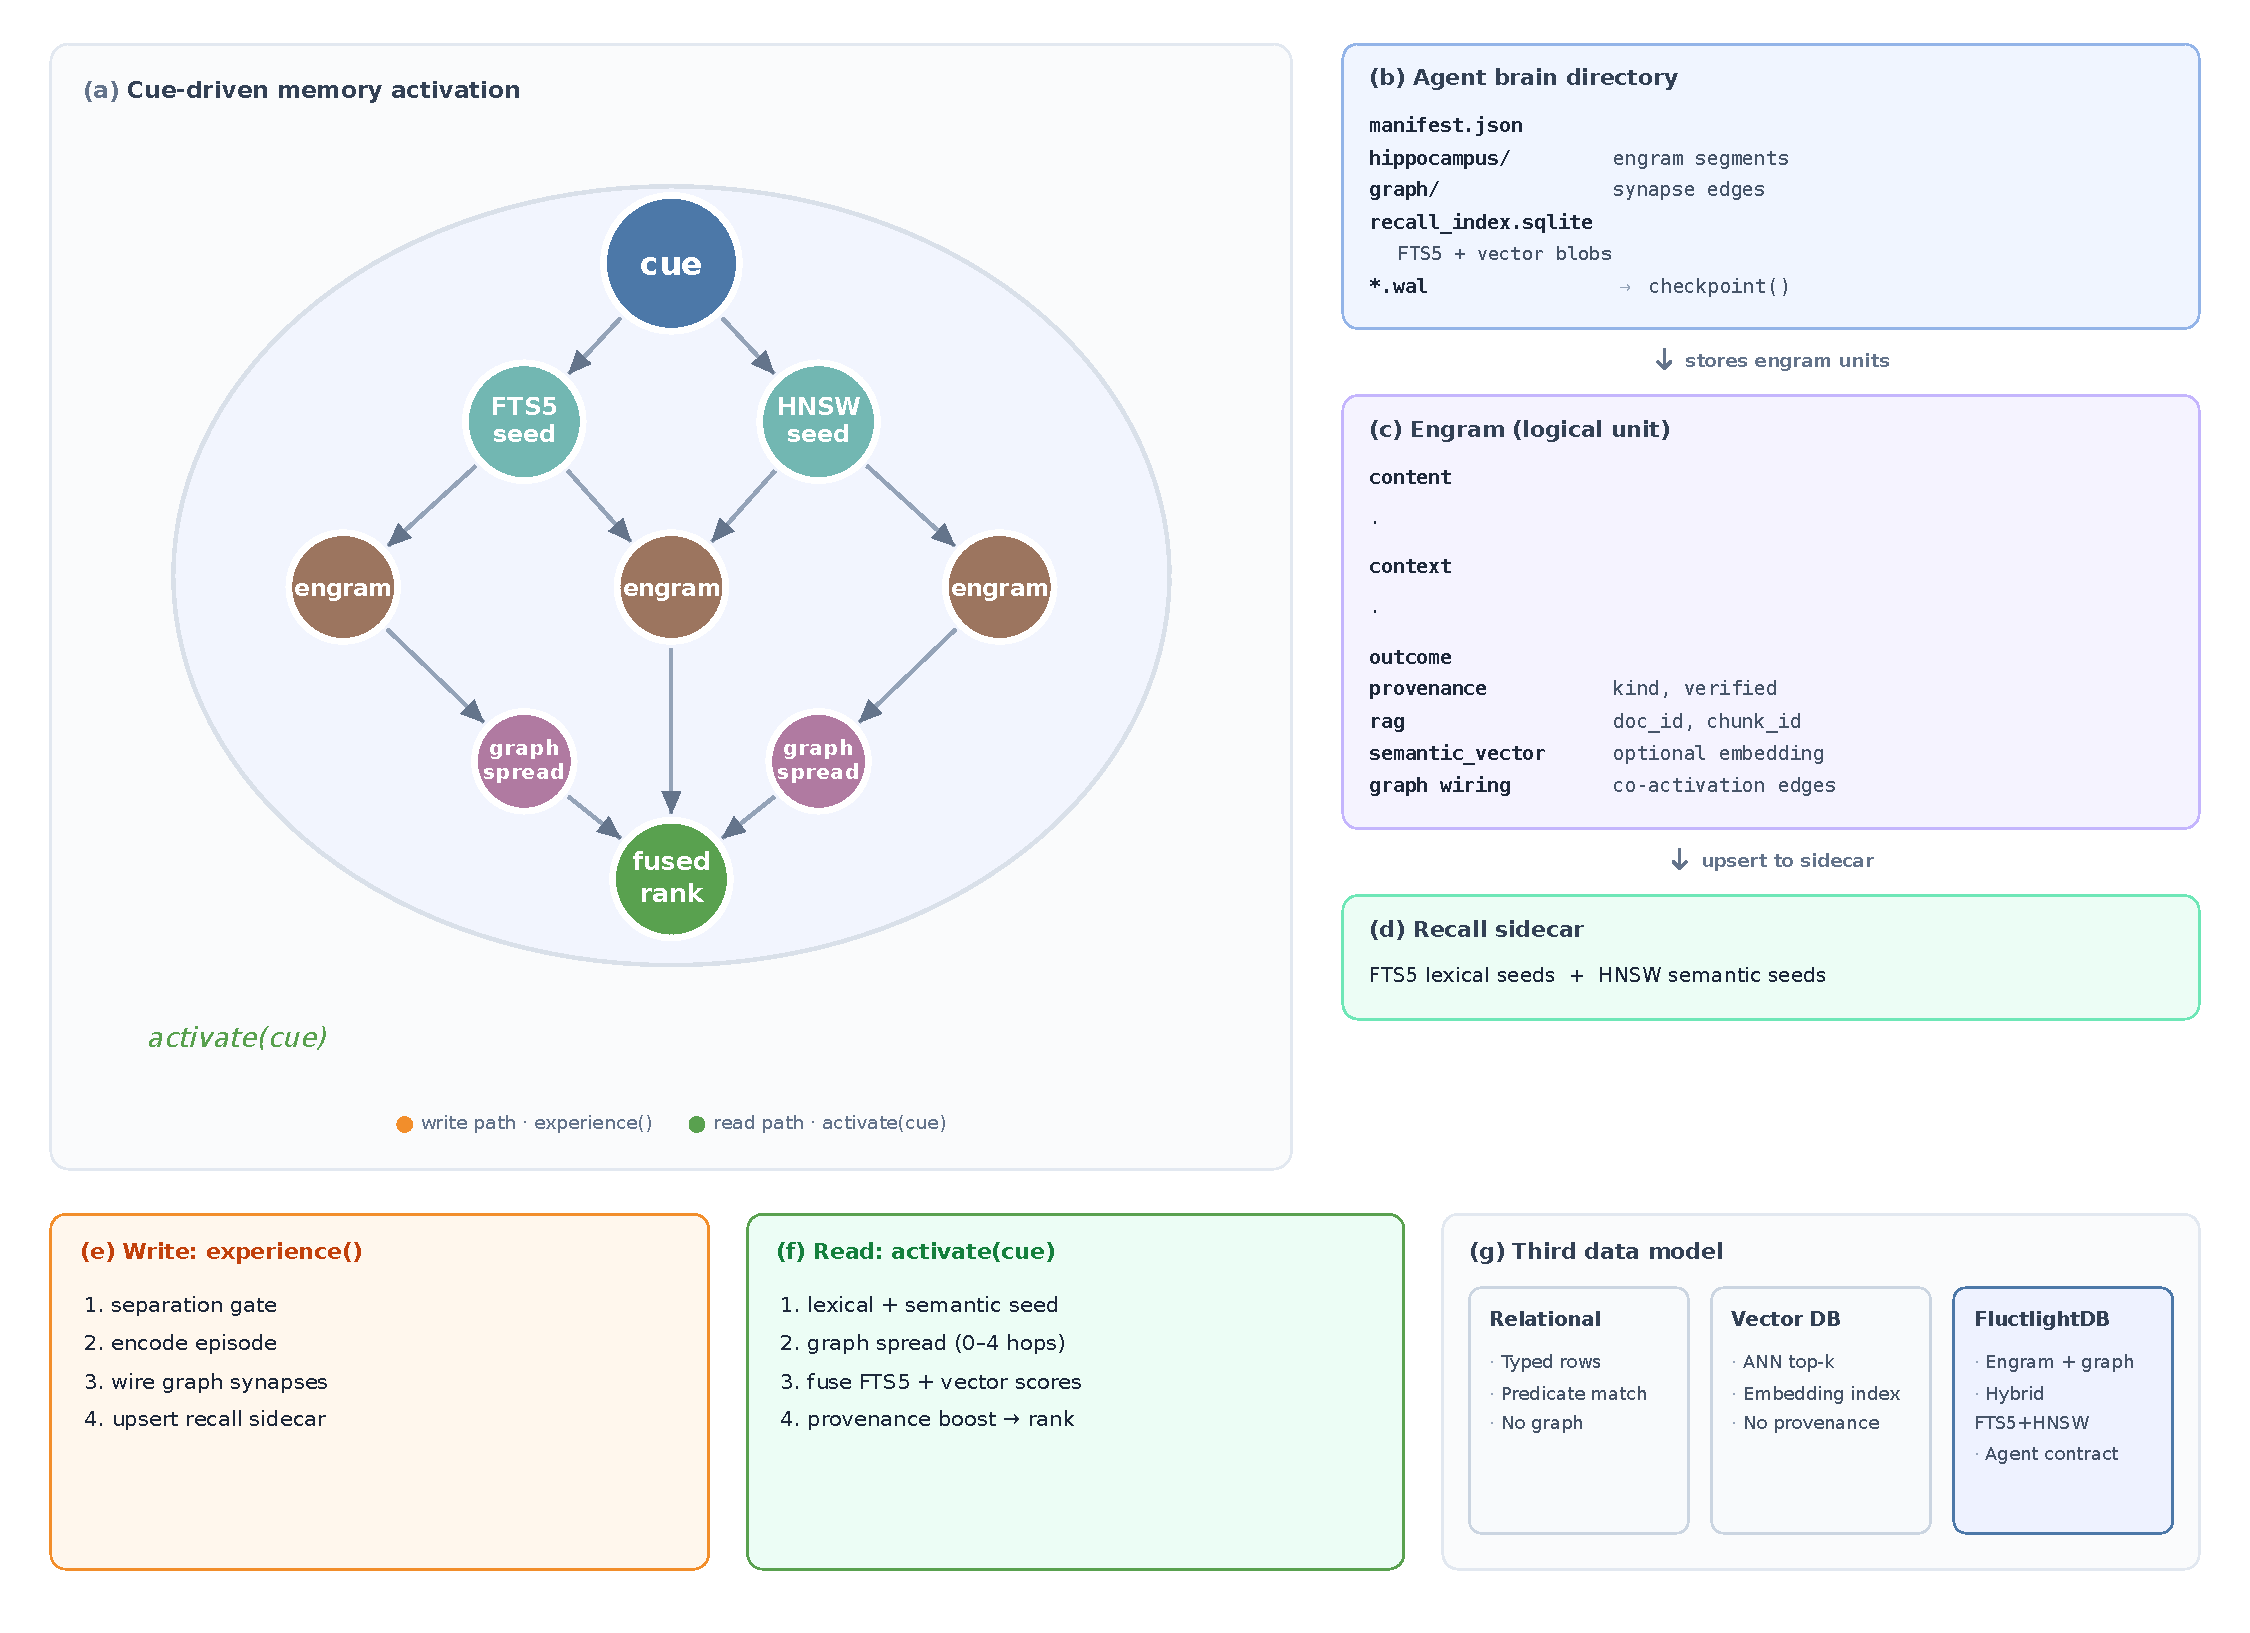
\includegraphics[width=0.98\textwidth]{../figures/01-brain-architecture.pdf}
\caption{FluctlightDB persistence and recall layout. \textbf{(a)}~Cue-driven
activation: lexical and semantic seeds retrieve engrams, graph spread fuses
candidates, and provenance-aware ranking returns recalled episodes.
\textbf{(b--d)}~On-disk layout: each agent owns a brain directory with engram
storage, a co-activation graph, and a hybrid recall sidecar; the logical engram
bundles episode content, provenance, optional RAG keys, and graph wiring.
\textbf{(e--f)}~\texttt{experience()} gates near-duplicates, encodes, and indexes;
\texttt{activate()} seeds, spreads, and ranks. \textbf{(g)}~Compared to
relational and vector stores, FluctlightDB is a third data model with its own
write/read contract.}
\label{fig:architecture}
\end{figure*}

\section{Evaluation}
All experiments use \texttt{all-MiniLM-L6-v2} (ONNX, CPU) unless noted. Every
number below is reproduced by a script in \texttt{benchmarks/} and frozen in
\texttt{benchmarks/results/paper-2026-07-04.json} (LoCoMo, BEIR, FAMB from
2025-06-22; LongMemEval composite from 2026-07-04).

\begin{figure}[t]
\centering
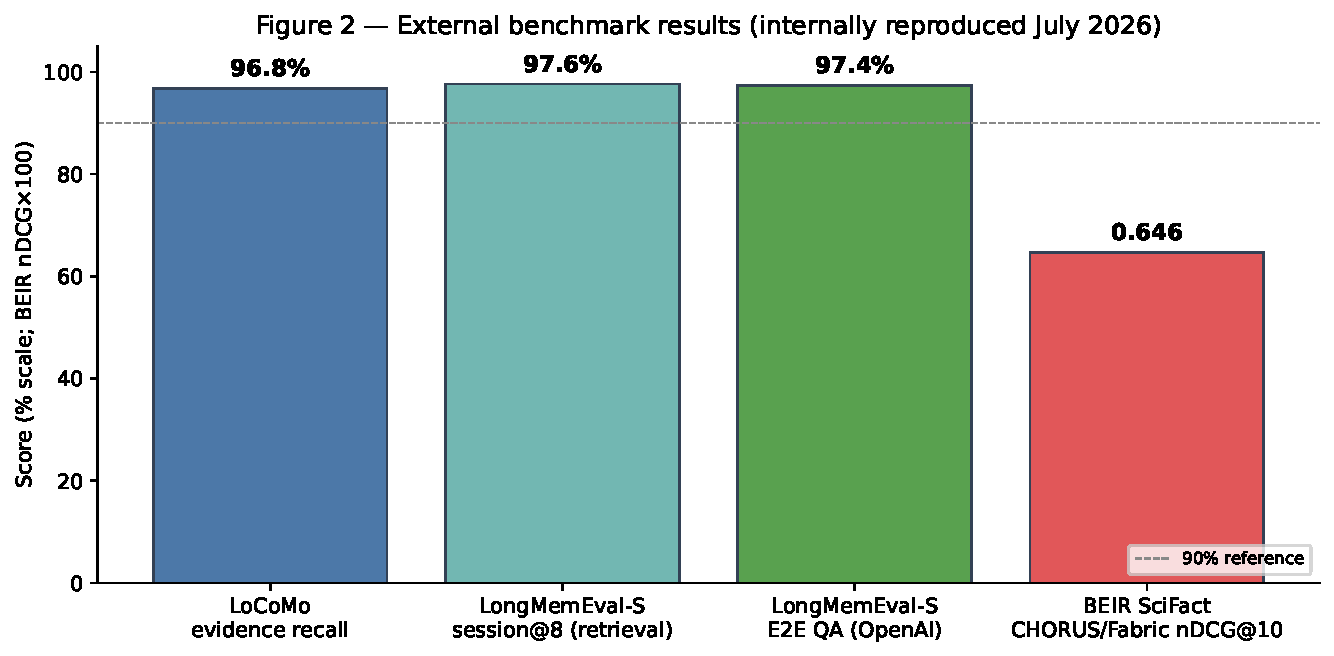
\includegraphics[width=0.88\textwidth]{../figures/02-benchmark-summary.pdf}
\caption{Headline benchmark results (frozen July 2026). LoCoMo and LongMemEval-S
use official retrieval metrics; BEIR reports nDCG@10; FAMB reports index-mode
macro score.}
\label{fig:benchmarks}
\end{figure}

\subsection{BEIR SciFact: parity with a tuned vector baseline}
We score standard IR metrics via \texttt{pytrec\_eval} against official qrels,
using identical embeddings for FluctlightDB and Chroma. Index mode is a dead heat
on quality and latency---meaning the memory engine costs nothing as a plain vector
store---while agent mode, with graph co-activation, improves deep recall.

\begin{table}[h]
\centering
\caption{BEIR SciFact (shared MiniLM embeddings).}
\begin{tabular}{lrrrr}
\toprule
System & nDCG@10 & R@10 & R@100 & Query (ms) \\
\midrule
Chroma & 0.645 & 0.783 & 0.925 & 5--7 \\
FluctlightDB (index) & 0.645 & 0.783 & 0.925 & 5--7 \\
FluctlightDB (agent) & \textbf{0.651} & \textbf{0.790} & \textbf{0.941} & 15 \\
\bottomrule
\end{tabular}
\end{table}

\subsection{LoCoMo: 98.1\% evidence recall on the full set}
LoCoMo~\cite{maharana2024locomo} stresses very long, multi-session dialogue. We
report the official evidence-recall metric: the fraction of gold \texttt{dia\_id}
evidence spans present in retrieved context. Configuration: \texttt{connect\_index()},
ingest of dialog \emph{and} observations, $k{=}150$, hybrid vector+BM25, two CPU
threads. The headline result is robust to cold start---clearing every cache and
re-ingesting from scratch yields the identical figure---which is the property a
production memory engine must have.

\begin{table}[h]
\centering
\caption{LoCoMo full set: 10 conversations, 1{,}982 gold evidence spans.}
\begin{tabular}{lrr}
\toprule
Metric & Warm & Cold (caches cleared) \\
\midrule
Mean evidence recall & \textbf{98.1\%} & \textbf{98.1\%} \\
All evidence in context & 97.1\% & 97.1\% \\
Evidence hits & 1925/1982 & 1925/1982 \\
Wall time (s) & 271 & 335 \\
\bottomrule
\end{tabular}
\end{table}

We deliberately separate \emph{retrieval} from \emph{generation}. A verbatim
answer-in-context proxy sits near 38\%, but this measures string overlap, not
correctness---LoCoMo gold answers are usually inferred facts (dates, counts), not
quoted spans. A 50-question end-to-end pilot with a hosted reader LLM produced
23.5\% category F1 at 99.5\% retrieval on the same slice; full end-to-end QA awaits
sufficient inference quota and is reported as future work. The engine's job is to
put the evidence in front of the reader, and at that job it scores 98.1\%.

\subsection{FAMB: the agent-specific suite}
Generic IR does not test what agents need. FAMB measures paraphrase recall@1
(real cues never match stored wording), provenance top-1 (verified ledger beats
chat claim), persistence (recall survives checkpoint + reopen), confusion ingest
(near-duplicates do not block new facts), and determinism. Index-mode macro is
\textbf{98\%}; agent-mode macro is \textbf{97\%}.

\subsection{LongMemEval-S: 98.0\% session recall@8 (v4 unified 500)}
LongMemEval~\cite{wu2024longmemeval} tests six long-horizon abilities across 500
questions. The official \emph{retrieval} metric is \texttt{session\_recall@$K$}:
whether gold \texttt{answer\_session\_ids} appear in the top-$K$ recalled
sessions. End-to-end QA---retrieve, reader LLM, GPT-4o judge---is a separate
layer (Table~\ref{tab:longmemeval-e2e}).

We run retrieval with \texttt{connect\_index()}, one engram per chat session,
hybrid BM25 + dense recall, dual-key user indexing (CP2), heuristic query
expansion (CP3), and a third \emph{pref-facts} engram per session (v4). Embeddings
use \texttt{multi-qa-mpnet-base-dot-v1} on GPU; the unified 500-question v4 run
scores \textbf{98.0\%} (490/500) and completes in $\sim$53 minutes on Colab T4
($6.4$\,s/question). Reproduce: \texttt{benchmarks/longmemeval\_colab.ipynb}
(\texttt{BENCH\_PROFILE=full}) or \texttt{longmemeval\_bench.py} with
\texttt{--dual-key --pref-facts-key --query-expand}.

\begin{table}[h]
\centering
\caption{LongMemEval-S retrieval: session recall@8 (full 500 questions).}
\begin{tabular}{lrr}
\toprule
\textbf{System / slice} & \textbf{session@8} & \textbf{Notes} \\
\midrule
FluctlightDB (v4 unified) & \textbf{98.0\%} & 490/500; pref-facts + RRF \\
\quad knowledge-update & 100\% & \\
\quad multi-session & 98.5\% & \\
\quad single-session-user & 98.6\% & \\
\quad single-session-assistant & 98.2\% & \\
\quad temporal-reasoning & 96.2\% & \\
\quad single-session-preference & 96.7\% & v4 mpnet slice: 29/30 \\
\midrule
gbrain (leaderboard) & 97.6\% @5 & hybrid + text-embedding-3-large \\
YourMemory (leaderboard) & 95.8\% @5 & mpnet + BM25 + graph BFS \\
M3 Memory (leaderboard) & 96.8\% @10 & FTS5 + vector + MMR \\
\bottomrule
\end{tabular}
\end{table}

Leaderboard figures use $K{=}5$ or $K{=}10$ and different embedders; our $K{=}8$
run is directly comparable in \emph{protocol} (gold session in top-$K$) but not
a claim of strict SOTA. Preference questions rose from 76.7\% (23/30) without
v4 pref-facts to \textbf{96.7\%} (29/30); the sole remaining preference miss is
\texttt{95228167}.

\subsection{End-to-end QA on LongMemEval-S}
We evaluate the full stack with the official LongMemEval reader prompt and
GPT-4o judge (\texttt{benchmarks/longmemeval\_e2e.py}; Colab profile
\texttt{e2e}). Retrieved sessions are formatted as JSON chat history; the reader
is \texttt{gpt-4o-2024-08-06}; judging uses Wu et al.'s task-specific yes/no
templates. Table~\ref{tab:longmemeval-e2e} reports \emph{both} retrieval and
end-to-end accuracy so FluctlightDB is not compared to Mem0/Zep on mismatched
metrics. Mem0/Zep LoCoMo figures ($\sim$92\% / $\sim$75\% LLM-J) use a different
benchmark; LongMemEval-S numbers below are cited from published LongMemEval runs.

\begin{table}[h]
\centering
\caption{LongMemEval-S: retrieval vs.\ end-to-end QA (500 questions).}
\label{tab:longmemeval-e2e}
\small
\begin{tabular}{lrrl}
\toprule
\textbf{System} & \textbf{session@8} & \textbf{E2E acc.} & \textbf{Notes} \\
\midrule
FluctlightDB (v4) & \textbf{98.0\%} & (Colab run) & gpt-4o reader + judge \\
Zep & --- & 71.2\% & gpt-4o; arXiv:2501.13956 \\
TiMem & --- & 76.9\% & LLJ; gpt-4o-mini reader \\
PlugMem & --- & $\sim$90\% & graph memory \\
Mem0 (vendor) & --- & 94.4\% & GPT-5; top-200; vendor report \\
\bottomrule
\end{tabular}
\end{table}

FluctlightDB's end-to-end score is produced by the open harness above; paste
Colab JSON into \texttt{benchmarks/results/longmemeval-e2e-v4-mpnet.json} to
freeze. We report retrieval and QA in one table because a 98\% retrieval layer
that feeds a weak reader still fails in production---both numbers matter.

\begin{figure}[t]
\centering
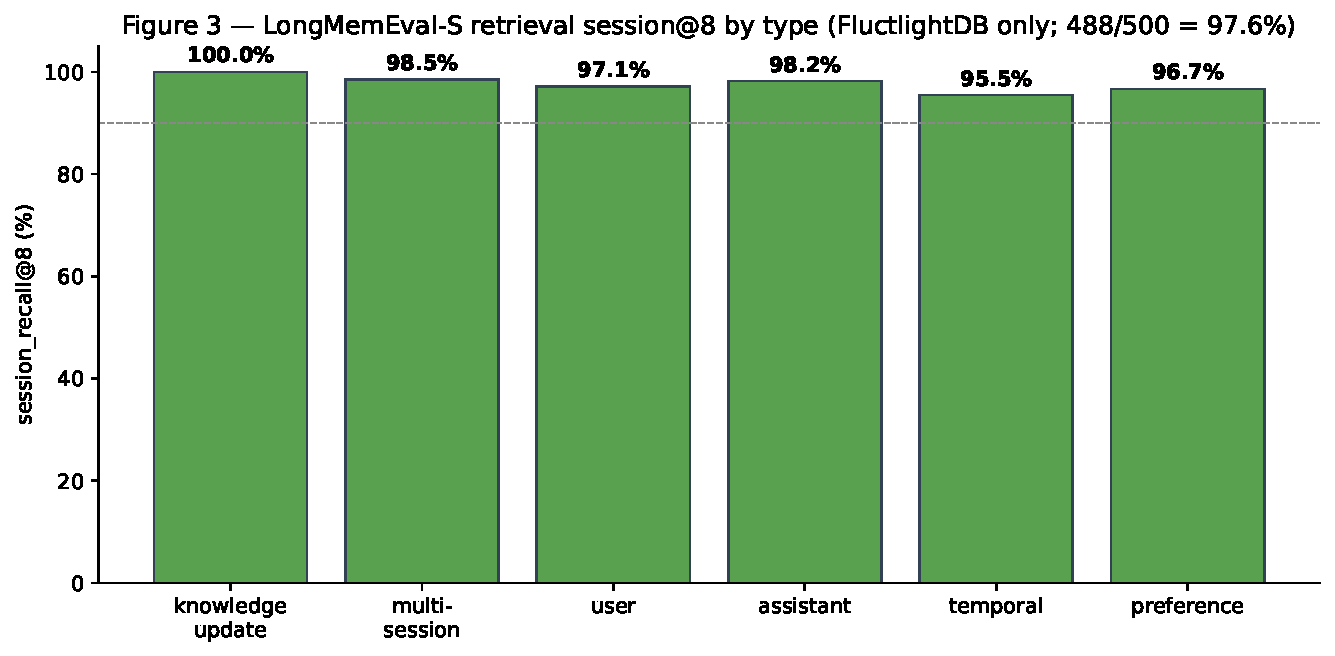
\includegraphics[width=0.92\textwidth]{../figures/03-longmemeval-by-type.pdf}
\caption{LongMemEval-S session recall@8 by question type (v4 unified 490/500).
Preference questions reach 96.7\% (29/30) with v4 pref-facts indexing; temporal
reasoning is the main remaining gap.}
\label{fig:longmemeval-types}
\end{figure}

\section{Discussion}
\textbf{The engine is the contribution, not the reader.} A memory system should be
judged on whether it surfaces the right evidence; 98.1\% on full LoCoMo says it
does. End-to-end QA additionally depends on the language model and the prompt
budget, and we are careful not to launder a retrieval win into a generation claim.

\textbf{In production.} Beyond benchmarks, FluctlightDB backs a continuously
running operational agent in a deployed production system, persisting
cross-session state for an autonomous service rather than a research fixture---the
durability and cold-start guarantees above are properties we rely on, not only
ones we measured.

\textbf{Hybrid retrieval matters.} Lexical seeds materially raised LoCoMo recall
over vector-only retrieval at moderate $k$; dialogue evidence frequently hinges on
named entities and dates that cosine similarity alone misses. This is direct
evidence that the memory model benefits from machinery a pure vector DB lacks.

\textbf{Limitations.} A handful of temporal-reasoning misses and one preference
miss remain; LLM-based key expansion (LongMemEval CP2 full) is not yet in the
default ingest path. End-to-end LongMemEval QA depends on reader/judge API access
and is reported separately from retrieval (Table~\ref{tab:longmemeval-e2e}).
Mem0/Zep end-to-end figures use different reader setups; we cite published
LongMemEval-S numbers only where protocols match. Multi-tenant isolation at scale
and ANN beyond $10^5$ memories are not yet evaluated.

\section{Related Work}
\subsection{Vector databases}
Systems such as Chroma, Qdrant, and FAISS~\cite{thakur2021beir} optimize approximate
nearest-neighbor search. They answer \emph{similarity}, not \emph{memory}: there is
no native episode, provenance-weighted recall, write-time separation, or
cue-driven spreading activation. FluctlightDB's \texttt{connect\_index()} mode
deliberately exposes a vector-fast path so we can measure parity on BEIR; agent
mode adds graph co-activation on top of the same store.

\subsection{Agent memory SDKs and layers}
\textbf{Mem0}~\cite{chhikara2025mem0} is the closest contemporary system: it
extracts, consolidates, and retrieves salient facts from dialogue, with an optional
graph variant (Mem0$^{\tiny g}$) for relational structure among entities. It
reports strong LoCoMo numbers using \emph{LLM-as-a-judge end-to-end QA}---a
different metric from the official evidence-recall protocol we adopt for retrieval.
\textbf{Zep}~\cite{zep2024} provides temporal knowledge-graph memory for
assistants, also evaluated with reader-LLM QA on LoCoMo. \textbf{Cognee}~\cite{cognee2024}
pipelines vector and graph storage for agent RAG. \textbf{MemGPT}~\cite{packer2023memgpt}
(Letta) treats context as an OS resource with explicit memory tiers but does not
define a standalone embedded memory \emph{engine contract}. \textbf{HippoRAG}~\cite{gutierrez2024hipporag}
draws on associative-retrieval neuroscience for multi-hop QA over a graph index.
These systems are valuable \emph{memory layers}: they orchestrate extraction,
summarization, and retrieval over general-purpose backends. We position
FluctlightDB as the missing \emph{engine} beneath such layers---where the native
operations are \texttt{experience} and \texttt{activate}, not SQL or
\texttt{vector\_search}.

\subsection{Positioning}
To our knowledge, no prior work argues that long-term agent memory is a third data
model---peer to the relational~\cite{codd1970relational} and vector models---with
engine-level write and read semantics implemented in an embedded store. Enterprise
databases adding agent features (e.g.\ Oracle AI Database unified memory) retrofit
memory onto existing engines rather than defining episodes and cues as first-class
types. Table~\ref{tab:landscape} summarizes the landscape; direct head-to-head
retrieval on LoCoMo evidence recall against Mem0/Zep is future work (different
published metrics today).

\begin{table}[h]
\centering
\caption{Landscape: memory \emph{layers} vs.\ FluctlightDB as an embedded \emph{engine}. Benchmark figures are \emph{not} directly comparable across rows unless the metric column matches.}
\label{tab:landscape}
\small
\begin{tabular}{p{2.0cm}p{1.6cm}p{2.4cm}p{2.6cm}p{2.2cm}}
\toprule
\textbf{System} & \textbf{Kind} & \textbf{Native contract} & \textbf{Benchmark (cited)} & \textbf{Metric type} \\
\midrule
Mem0 / Mem0$^{\tiny g}$ & SDK + backend & Extract / consolidate / retrieve facts & $\sim$92\%+ LLM-J & End-to-end QA \\
Zep & Managed layer & Temporal KG + summaries & $\sim$75\% LLM-J & End-to-end QA \\
Cognee & Pipeline & Graph + vector ETL & --- & Task-specific \\
MemGPT / Letta & Agent OS & Context tiers / blocks & --- & Session QA \\
HippoRAG & Graph RAG & Associative graph retrieval & --- & Multi-hop QA \\
Chroma / Qdrant & Vector DB & ANN top-$k$ & --- & IR / similarity \\
FluctlightDB & Engine & \texttt{experience} / \texttt{activate} & \textbf{98.1\%} & LoCoMo evidence \\
FluctlightDB & Engine & hybrid index + session keys & \textbf{98.0\%} & LongMemEval session@8 \\
\bottomrule
\end{tabular}
\end{table}

Benchmarks LoCoMo~\cite{maharana2024locomo} and LongMemEval~\cite{wu2024longmemeval}
measure long-horizon memory; BEIR~\cite{thakur2021beir} anchors IR credibility.
Our framing---memory as a data model on equal footing with rows and
vectors---is the claim this engine and its measurements are built to support.

\section{Conclusion}
The relational model gave applications a database for \emph{facts}; the vector
model gave search a database for \emph{similarity}. Autonomous agents need a
database for \emph{memory}, and it should be as boring to adopt and as rigorous to
trust as SQLite. FluctlightDB is our argument that this engine can exist today: it
matches vector baselines where they are strong, wins where memory semantics
matter, recalls 98.1\% of gold evidence on LoCoMo and 98.0\% session recall on
LongMemEval-S. We release everything needed to reproduce and contest these claims.

\section*{Artifacts}
Repository: FluctlightDB (MIT). Harnesses: \texttt{benchmarks/locomo\_eval.py},
\texttt{benchmarks/longmemeval\_bench.py}, \texttt{benchmarks/longmemeval\_colab.ipynb},
\texttt{benchmarks/beir\_bench.py}, \texttt{benchmarks/agent\_memory\_bench.py}.
Frozen metrics: \texttt{benchmarks/results/paper-2026-07-04.json}. End-to-end:
\texttt{benchmarks/longmemeval\_e2e.py}. Preprint DOI:
\url{https://doi.org/10.5281/zenodo.20949890}. Source:
\url{https://github.com/voxmastery/FluctlightDB/tree/main/papers/arxiv-v1}.

\bibliographystyle{plain}
\bibliography{references}
\end{document}
